\documentclass[11pt,a4paper,twocolumn]{article}

\usepackage{caption}
\usepackage{float}
\usepackage{geometry}
\usepackage{graphicx}
\usepackage{listings}
\usepackage{url}

\captionsetup[figure]{name=Figura}
\def\refname{Referencias}
\geometry{margin=1in}
\setlength{\columnsep}{0.5in}

\author{V. Blanco, A. Navarro, J. Ferreira \& T. Oganesyan}
\date{22 de junio de 2026}
\title{\textbf{Ataque a la Pila por \textit{Stack Smashing} en Linux i386}}

\begin{document}
\maketitle

\section{Resumen}
Esta memoria está dedicada a analizar un ataque por \textit{stack smashing} en un sistema Linux. Concretamente, la víctima es un sistema para procesadores i386, lo que será importante en cuanto al lenguaje ensamblador a analizar.

Para ello, se ha hecho uso del lenguaje de programación C, la herramienta \textit{make} y el compilador y debugger de GNU, todo bajo un subsistema Docker.

\section{Código Vulnerable}
La vulnerabilidad explotada es un \textit{buffer overflow} que se da por la naturaleza del código. Las siguientes líneas de la función \texttt{smash()} (fichero \texttt{stsmash.c}) son clave:

\begin{lstlisting}[language=C]
char buffer[500];
read(0, buffer, 700);
\end{lstlisting}

Como se puede ver en la declaración del buffer y la llamada a la función \texttt{read()}, se permite que el usuario introduzca más datos de los que el buffer puede alojar.

\section{Metodología de ataque}
El ataque pretende conseguir desbordar el buffer alojado en el stack. Para ello, se aprovecha el hecho de que la función \texttt{read()} no comprueba límites en el buffer de ninguna manera.

Conociendo el código, es fácil darse cuenta de que, como $700>500$, podemos sobrepasar el límite superior del buffer. Sin embargo, si se considerara el programa como una caja negra (sin tener acceso al código), habría que realizar un análisis profundo, descompilando el programa.

\section{Análisis con GDB}
Para realizar el análisis real del código a partir del binario compilado, utilizamos el debugger de GNU (GDB) y algunas instrucciones.

Comenzamos desensamblando las funciones del programa. Todo programa a bajo nivel tiene una función principal, \texttt{main()}. Empezaremos examinándo dicha función. Véase la Figura 1.

\begin{figure}[H]
\centering
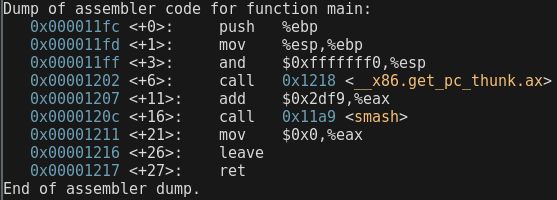
\includegraphics[scale=0.40]{images/ss-disa-1.png}
\caption{Desensamblado de la función \texttt{main}.}
\label{disassemble main}
\end{figure}

A partir de este código ensamblador, descubrimos una cierta función de nombre \textit{smash}. La desensamblamos. Véase la Figura 2.

\begin{figure}[H]
\centering
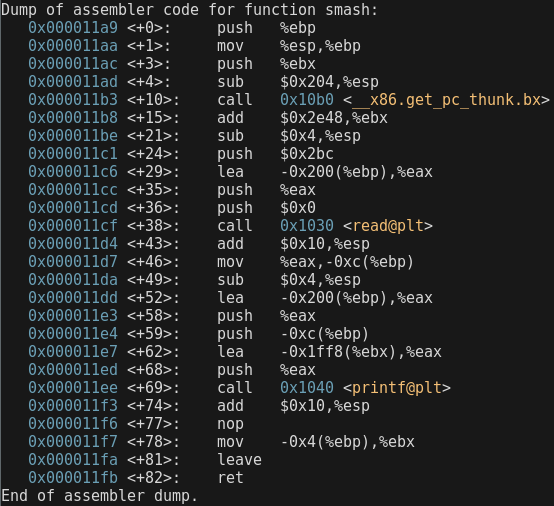
\includegraphics[scale=0.38]{images/ss-disa-2.png}
\caption{Desensamblado de la función \texttt{smash}.}
\label{disassemble smash}
\end{figure}

Situamos paradas (\textit{breakpoints}) en ciertas posiciones de la función \texttt{smash()} descubierta. Véase la Figura 3.

\begin{figure}[H]
\centering
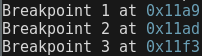
\includegraphics[scale=0.80]{images/ss-break-0.png}
\caption{Posiciones de parada.}
\label{breakpoints}
\end{figure}

Después de poner las paradas, correremos el programa compilado con la instrucción del debugger \textit{run}, pero introduciéndole un fichero pregenerado que contiene $700$ 'A's. Esto es, \texttt{run < input.txt}.

Tras la primera parada, leeremos el contenido del registro \texttt{\$ebp}, que guarda el puntero a la pila desde que se llama a la función \texttt{smash} hasta que esta retorna. Véase la Figura 4.

\begin{figure}[htp]
\centering
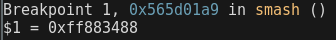
\includegraphics[scale=0.60]{images/ss-break-1.png}
\caption{Contenidos del registro \$ebp nada más llamar a la función \texttt{smash}.}
\label{stack pointer}
\end{figure}

A continuación, mostraremos los contenidos de los primeros $400$ bytes de la pila, antes de que ocurra el smashing. Véase la Figura 5.

\begin{figure}[htp]
\centering
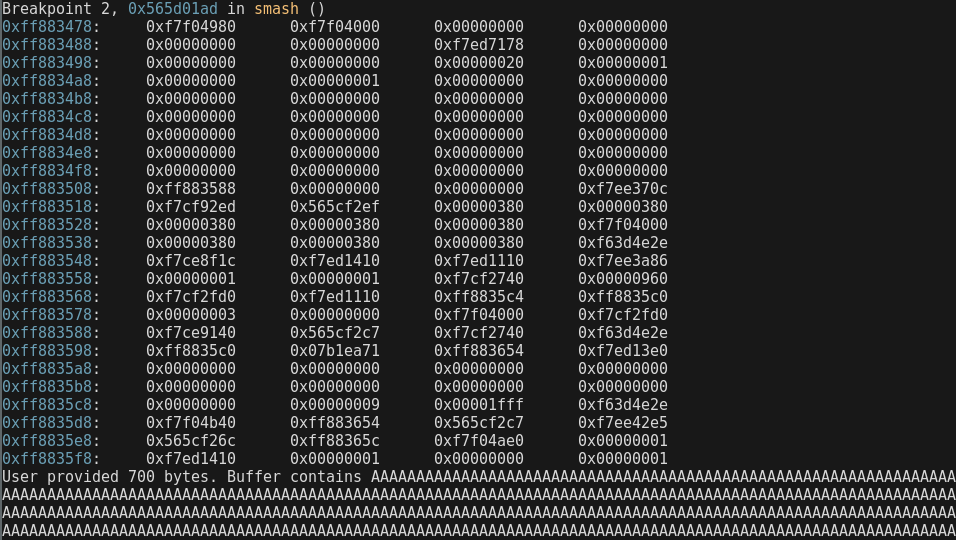
\includegraphics[scale=0.22]{images/ss-break-2.png}
\caption{Primeros $400$ bytes de la pila, antes del \textit{smash}.}
\label{stack before smash}
\end{figure}

Antes del ataque, la pila está limpia y correcta, como se esperaría de un programa bien compilado. Veamos qué ocurre tras continuar con el debugging. Véase la Figura 6.

\begin{figure}[htp]
\centering
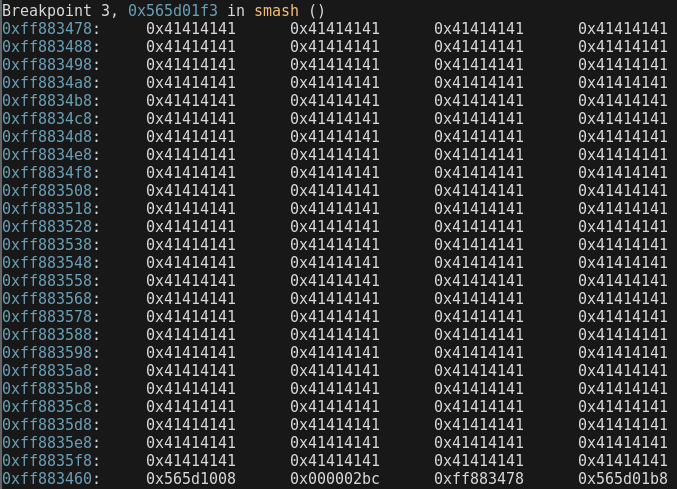
\includegraphics[scale=0.31]{images/ss-break-3.png}
\caption{Siguientes $400$ bytes de la pila, después del \textit{smash}.}
\label{stack after smash}
\end{figure}

Resulta que, tras introducirle más 'A's de las que puede almacenar, hemos logrado nuestro objetivo: sobreescribir la pila.

\section{Resultados}
Este ataque es sencillamente una prueba de que, en sistemas algo más antiguos a los actuales, se pueden realizar sobreescrituras indeseadas (por parte del usuario) con binarios muy sencillos.

Sin embargo, esto se puede llegar a utilizar para realizar inyecciones de código arbitrario en la pila de otros programas en ejecución. Explotar esa vulnerabilidad podría llevar de sencillos ataques de denegación de servicio (DoS), a ransomwares (virus que encriptan ficheros) o incluso robo de datos por envío remoto, entre otros.

\section{Mitigaciones}
Los compiladores de hoy en día presentan multitud de herramientas y niveles de análisis de código internos para tratar de evitar este tipo de ataques.

Por ejemplo, cuentan con el ASLR (\textit{Address Space Layout Randomisation}), que, en base a aleatorizar las zonas de memoria donde se ejecuta un programa cada vez, puede evitar accesos directos a ciertas partes del sistema \cite{wiki:aslr}; o la flag \texttt{-D\_FORTIFY\_SOURCE}, desarrollada por Red Hat para la GCC, que intenta evitar la ejecución de código inyectado a partir de cadenas de caracteres \cite{wiki:fortsrc}.

\section{Conclusión}
Aunque la mayor parte de los sistemas instalados hoy en día sean fuertes o casi invulnerables a este tipo de ataque, no hay que olvidar que existen grandes cantidades de servidores utilizando versiones desactualizadas paquetes de compiladores y el kernel de Linux. Por tanto, esta es una vulnerabilidad que los equipos azules de, sobre todo, empresas y organizaciones grandes deben de tener en cuenta a la hora de ejecutar programas en sus servidores.

\begin{thebibliography}{999}

\bibitem{wiki:aslr}
Wikipedia Contributors,
\textit{Address space layout randomization},
\url{https://en.wikipedia.org/w/index.php?title=Address_space_layout_randomization&oldid=1355882436},
(Accesed: June 22, 2026).

\bibitem{wiki:fortsrc}
Wikipedia Contributors,
\textit{Exec Shield},
\url{https://en.wikipedia.org/w/index.php?title=Exec_Shield&oldid=1268856958},
(Accessed: June 22, 2026).

\end{thebibliography}

\end{document}